\setAuthor{Hans Daniel Kaimre}
\setRound{piirkonnavoor}
\setYear{2019}
\setNumber{G 6}
\setDifficulty{6}
\setTopic{Elektriahelad}

\prob{Kondensaator}
Kondensaatorit laetakse kõrvaloleva skeemi järgi alalisvooluallikast pingega $U=\SI{12}{\V}$. Skeemis olevate takistite takistused on vastavalt $R_1=\SI{1}{\kilo\ohm}$, $R_2=\SI{2}{\kilo\ohm}$ ning $R_3=\SI{3}{\kilo\ohm}$. Millise maksimaalse pingeni on kondensaatorit niimoodi võimalik laadida? 
\begin{center}
  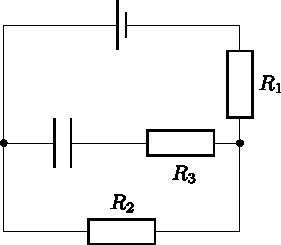
\includegraphics[width = 0.40\linewidth]{2019-v2g-06-yl.pdf}
\end{center}\hint
Maksimaalse pingeni laetud kondensaatorit vool ei läbi. Vastasel juhul ei oleks tegu maksimaalse pingega. Järelikult ei läbi ka takistit $R_3$ vool.\solu
Pinge kondensaatoril on maksimaalne siis, kui seda vool ei läbi. Sellisel juhul on ka takistit $R_3$ läbiv vool ning omakorda ka pingelang null. See tähendab, et pinge kondensaatori klemmidel on võrdne pingega takistil $R_2$. Viimase leiame Ohmi seadusest:
\begin{align*}
  U_2&=I_2R_2, \quad I_2=\frac{U}{R_1+R_2} \Rightarrow\\
  U_C&=U_2=\frac{U}{R_1+R_2}R_2 = \SI{8}{V}.
\end{align*}\probend